%%%%%%%%%%%%%%%%%%%%%%%%%%%%%%%%%%%%%%%%%
% University Assignment Title Page 
% LaTeX Template
% Version 1.0 (27/12/12)
%
% This template has been downloaded from:
% http://www.LaTeXTemplates.com
%
% Original author:
% WikiBooks (http://en.wikibooks.org/wiki/LaTeX/Title_Creation)
%
% License:
% CC BY-NC-SA 3.0 (http://creativecommons.org/licenses/by-nc-sa/3.0/)
%
%%%%%%%%%%%%%%%%%%%%%%%%%%%%%%%%%%%%%%%%%
%\title{Title page with logo}
%----------------------------------------------------------------------------------------
%	PACKAGES AND OTHER DOCUMENT CONFIGURATIONS
%----------------------------------------------------------------------------------------

\documentclass[12pt]{article}
\usepackage[english]{babel}
\usepackage[utf8x]{inputenc}
\usepackage{natbib}
\usepackage{amsmath}
\usepackage[colorinlistoftodos]{todonotes}
\usepackage{listings}
\usepackage{color}
\usepackage[explicit]{titlesec}
\usepackage{url}
\usepackage{subfig}
\usepackage{graphicx}
\usepackage{grffile}

\titleformat{\section}{\normalfont\Large\bfseries}{Experiment \thesection}{1em}{}

\definecolor{dkgreen}{rgb}{0,0.6,0}
\definecolor{gray}{rgb}{0.5,0.5,0.5}
\definecolor{mauve}{rgb}{0.58,0,0.82}

\begin{document}

\begin{titlepage}

\newcommand{\HRule}{\rule{\linewidth}{0.5mm}} % Defines a new command for the horizontal lines, change thickness here

\center % Center everything on the page
 
%----------------------------------------------------------------------------------------
%	HEADING SECTIONS
%----------------------------------------------------------------------------------------

\textsc{\LARGE University of St Andrews}\\[1.5cm] % Name of your university/college
\textsc{\Large CS4203 Coursework 2}\\[0.5cm] % Major heading such as course name
\textsc{\large }\\[0.5cm] % Minor heading such as course title

%----------------------------------------------------------------------------------------
%	TITLE SECTION
%----------------------------------------------------------------------------------------

\HRule \\[0.4cm]
{ \huge \bfseries Security Tools}\\[0.4cm] % Title of your document
\HRule \\[1.5cm]
 
%----------------------------------------------------------------------------------------
%	AUTHOR SECTION
%----------------------------------------------------------------------------------------


\Large \emph{Author:}\\
 \textsc{150008022}\\[3cm] % Your name

%----------------------------------------------------------------------------------------
%	DATE SECTION
%----------------------------------------------------------------------------------------

{\large \today}\\[2cm] % Date, change the \today to a set date if you want to be precise

%----------------------------------------------------------------------------------------
%	LOGO SECTION
%---------------------------------------------------------------------------------------


\includegraphics[width = 3.1cm]{images/standrewslogo.png}
 
%----------------------------------------------------------------------------------------

\vfill % Fill the rest of the page with whitespace

\end{titlepage}

\part*{Goal}

The goal of this practical was to use and evaluate common tools and techniques used in security: steganography and penetration testing.

\part{Steganography}

Least Significant Bit (LSB) steganography - specifically LSB1 - involves replacing the last bit of each byte of an image file (called the cover image) with a bit from the message to be hidden. For example, if each character in the message requires a single byte, then it can be hidden in 8 bytes of the cover image. If we instead use the two least significant bits, we can half the image size needed to mask our message, but this can result in more obvious distortion in the original image. The message being hidden doesn't necessarily have to be text either, images can be masked using other images as well.

The goal of steganography is not to make the message impossible to understand, but to instead make its presence unknown to all but those that know to look for it. Because of this, we can focus our attention on what human vision will not notice so that we can exploit it to efficiently mask messages. 

Experiment \ref{comparingimages} compares various images after LSB steganography is applied. In experiment \ref{rgbvsycbcr}, a comparison is made between LSBs effectiveness with RGB and a more perceptually focused format: YCbCr.

\section{Effect of Spatial Frequencies on Hiding with LSB in RGB} \label{comparingimages}

\subsection{Introduction}
Images can contain a range of spatial frequencies. High frequency images show fine details, whilst low frequency images consist of smoother transitions between dark and light (See figure \ref{fig:spacefreq}). In this experiment, the effect of LSB on images of varying spatial frequencies is compared, using an online image steganography tool \cite{imagesteg}.

\begin{figure}%
    \centering
    \subfloat[High spatial frequency image]{{\includegraphics[width=5cm]{"images/lsbrgb/face_high_SF"} }}%
    \qquad
    \subfloat[Low spatial frequency image]{{\includegraphics[width=5cm]{"images/lsbrgb/face_low_SF"} }}%
    \caption{Comparison of spatial frequencies in images \cite{spatialfreq}}%
    \label{fig:spacefreq}%
\end{figure}

\subsection{Aims}

The aims of this experiment are:
\begin{enumerate}
	\item to determine whether a high, medium, or low frequency image is a better candidate for a cover file. \label{stegaimcover}
	\item to determine if high or low frequency images are most effective as the hidden images. \label{stegaimhidden}
\end{enumerate}

\subsection{Methods}
In order to reduce the number of variables in this experiment and simplify masking one image in another, the images used were all cropped and scaled to the size of $640\times396$ pixels. Three images were used that contained either low, medium or high values spatial frequency components.
	 A Matlab\textsuperscript{\textregistered} script was written (\textit{showDCT.m}) that converted the images to grayscale and used Discrete Cosine Transform to show the distribution of spatial frequencies. The images used and their spatial frequencies are shown in Figures \ref{fig:highfreq} to \ref{fig:lowfreq}. The DCT plots show the lowest frequencies in the top left and the highest frequencies in the bottom right. 

      \begin{figure}[!htb]
        \center{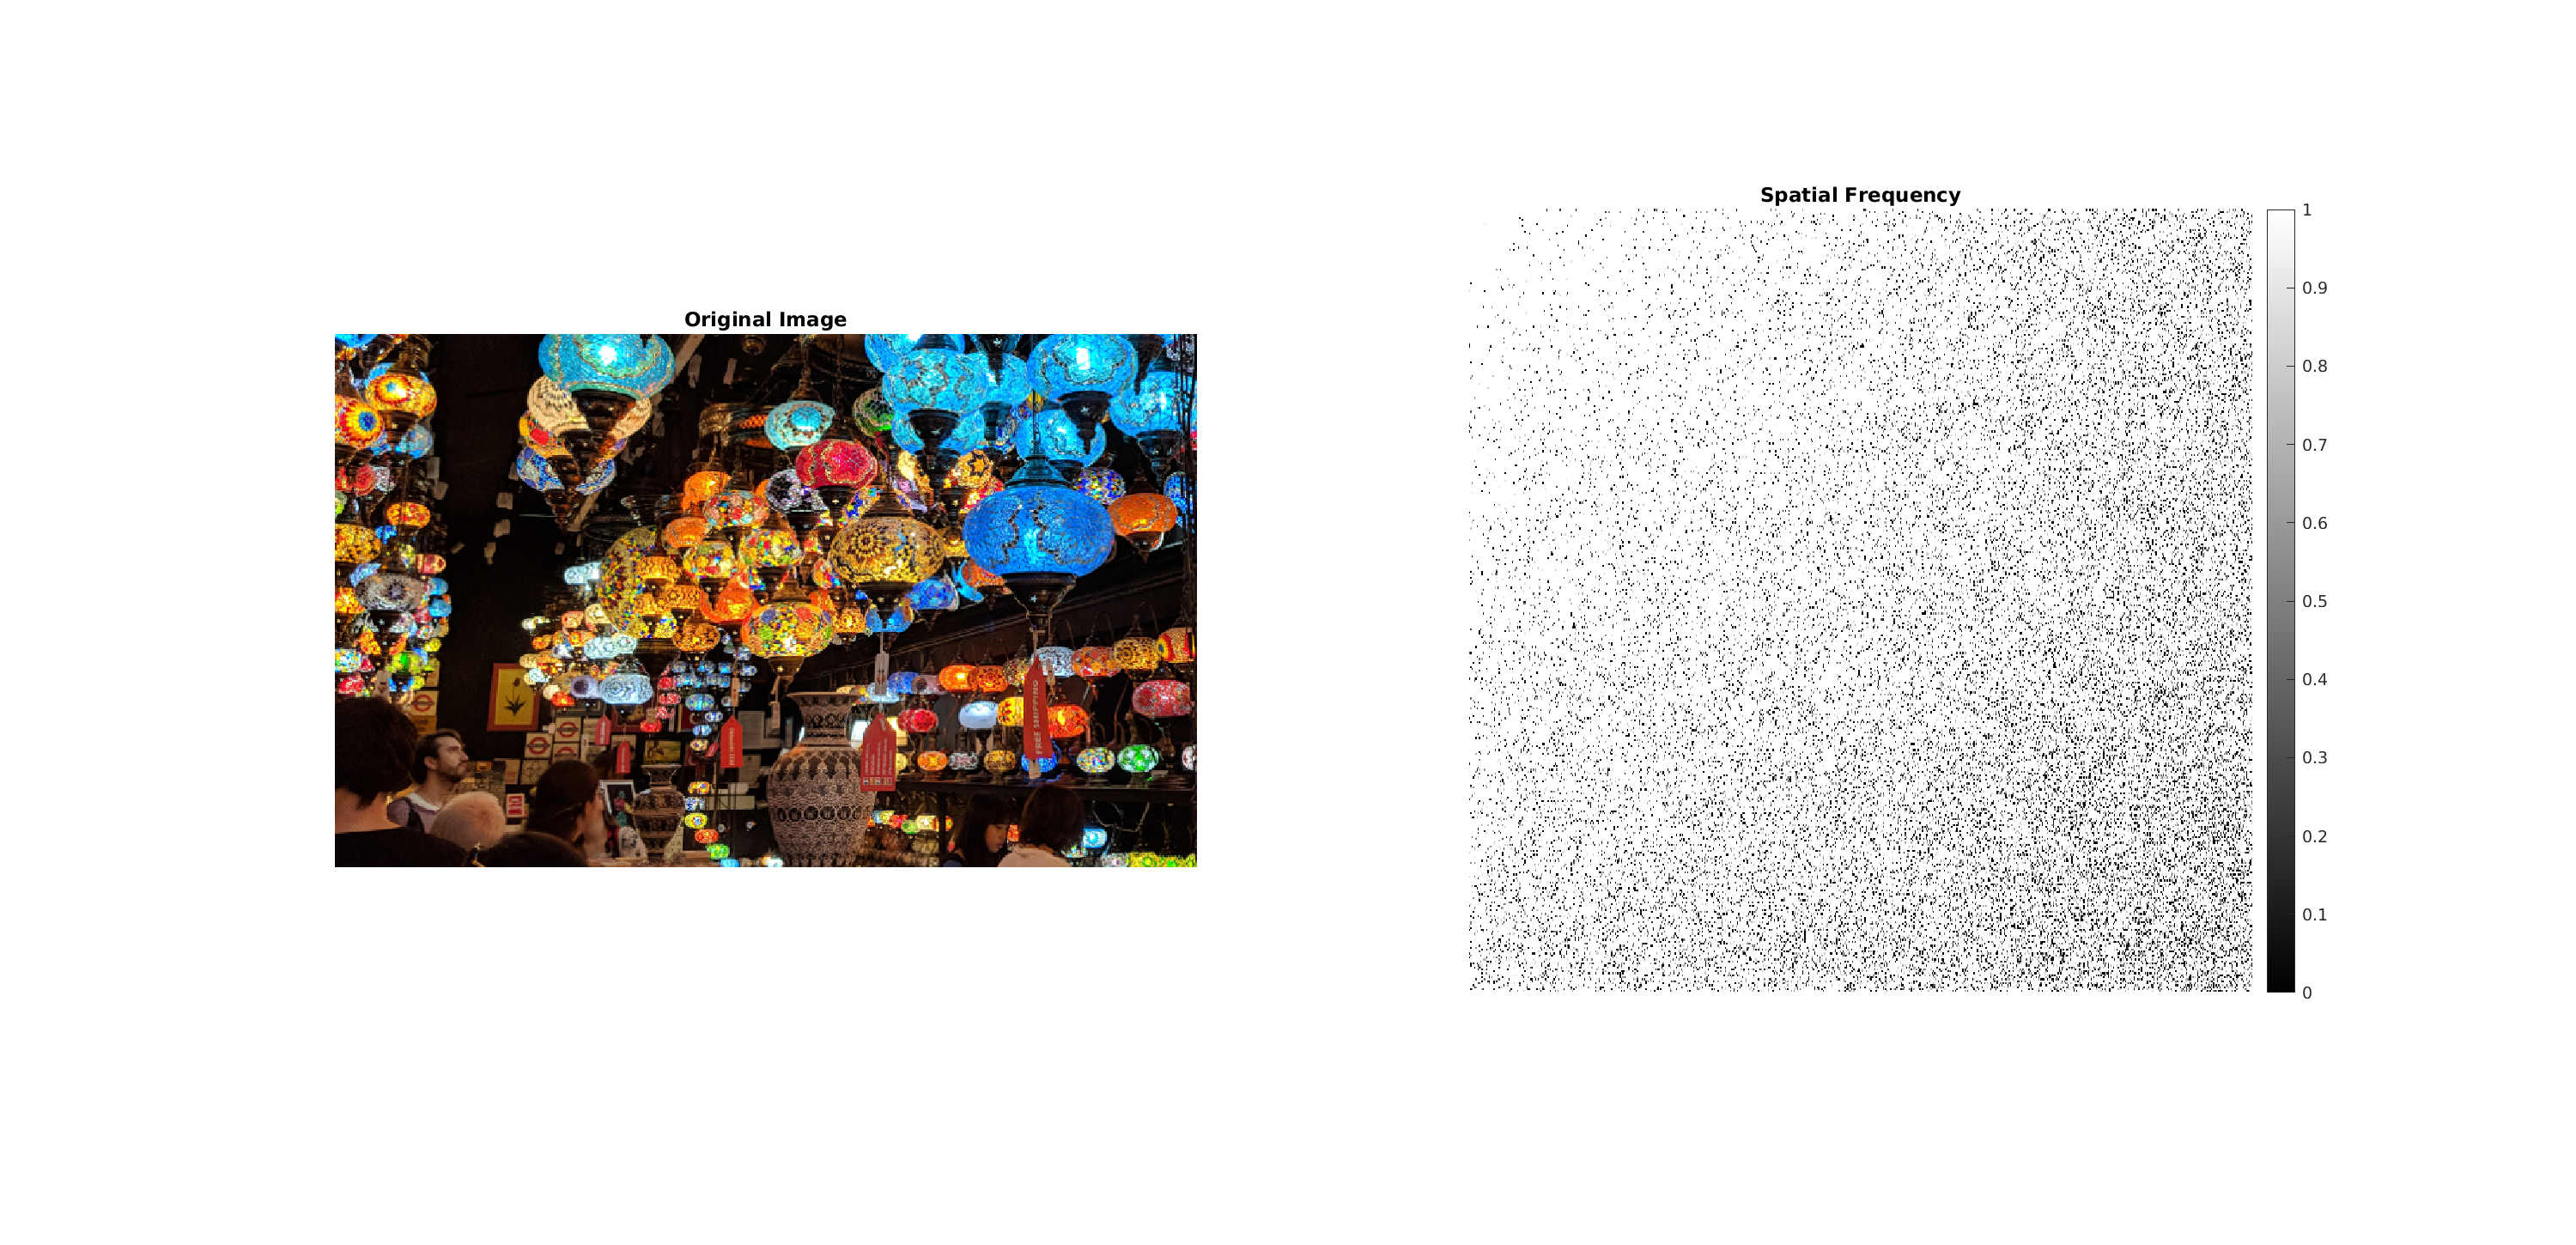
\includegraphics[width=\textwidth]
        {images/lsbrgb/dct/colourful_highfreq_dct.png}}
        \caption{\label{fig:highfreq} High frequency image (left) and spatial frequency distribution (right).}
      \end{figure}
      \begin{figure}[!htb]
        \center{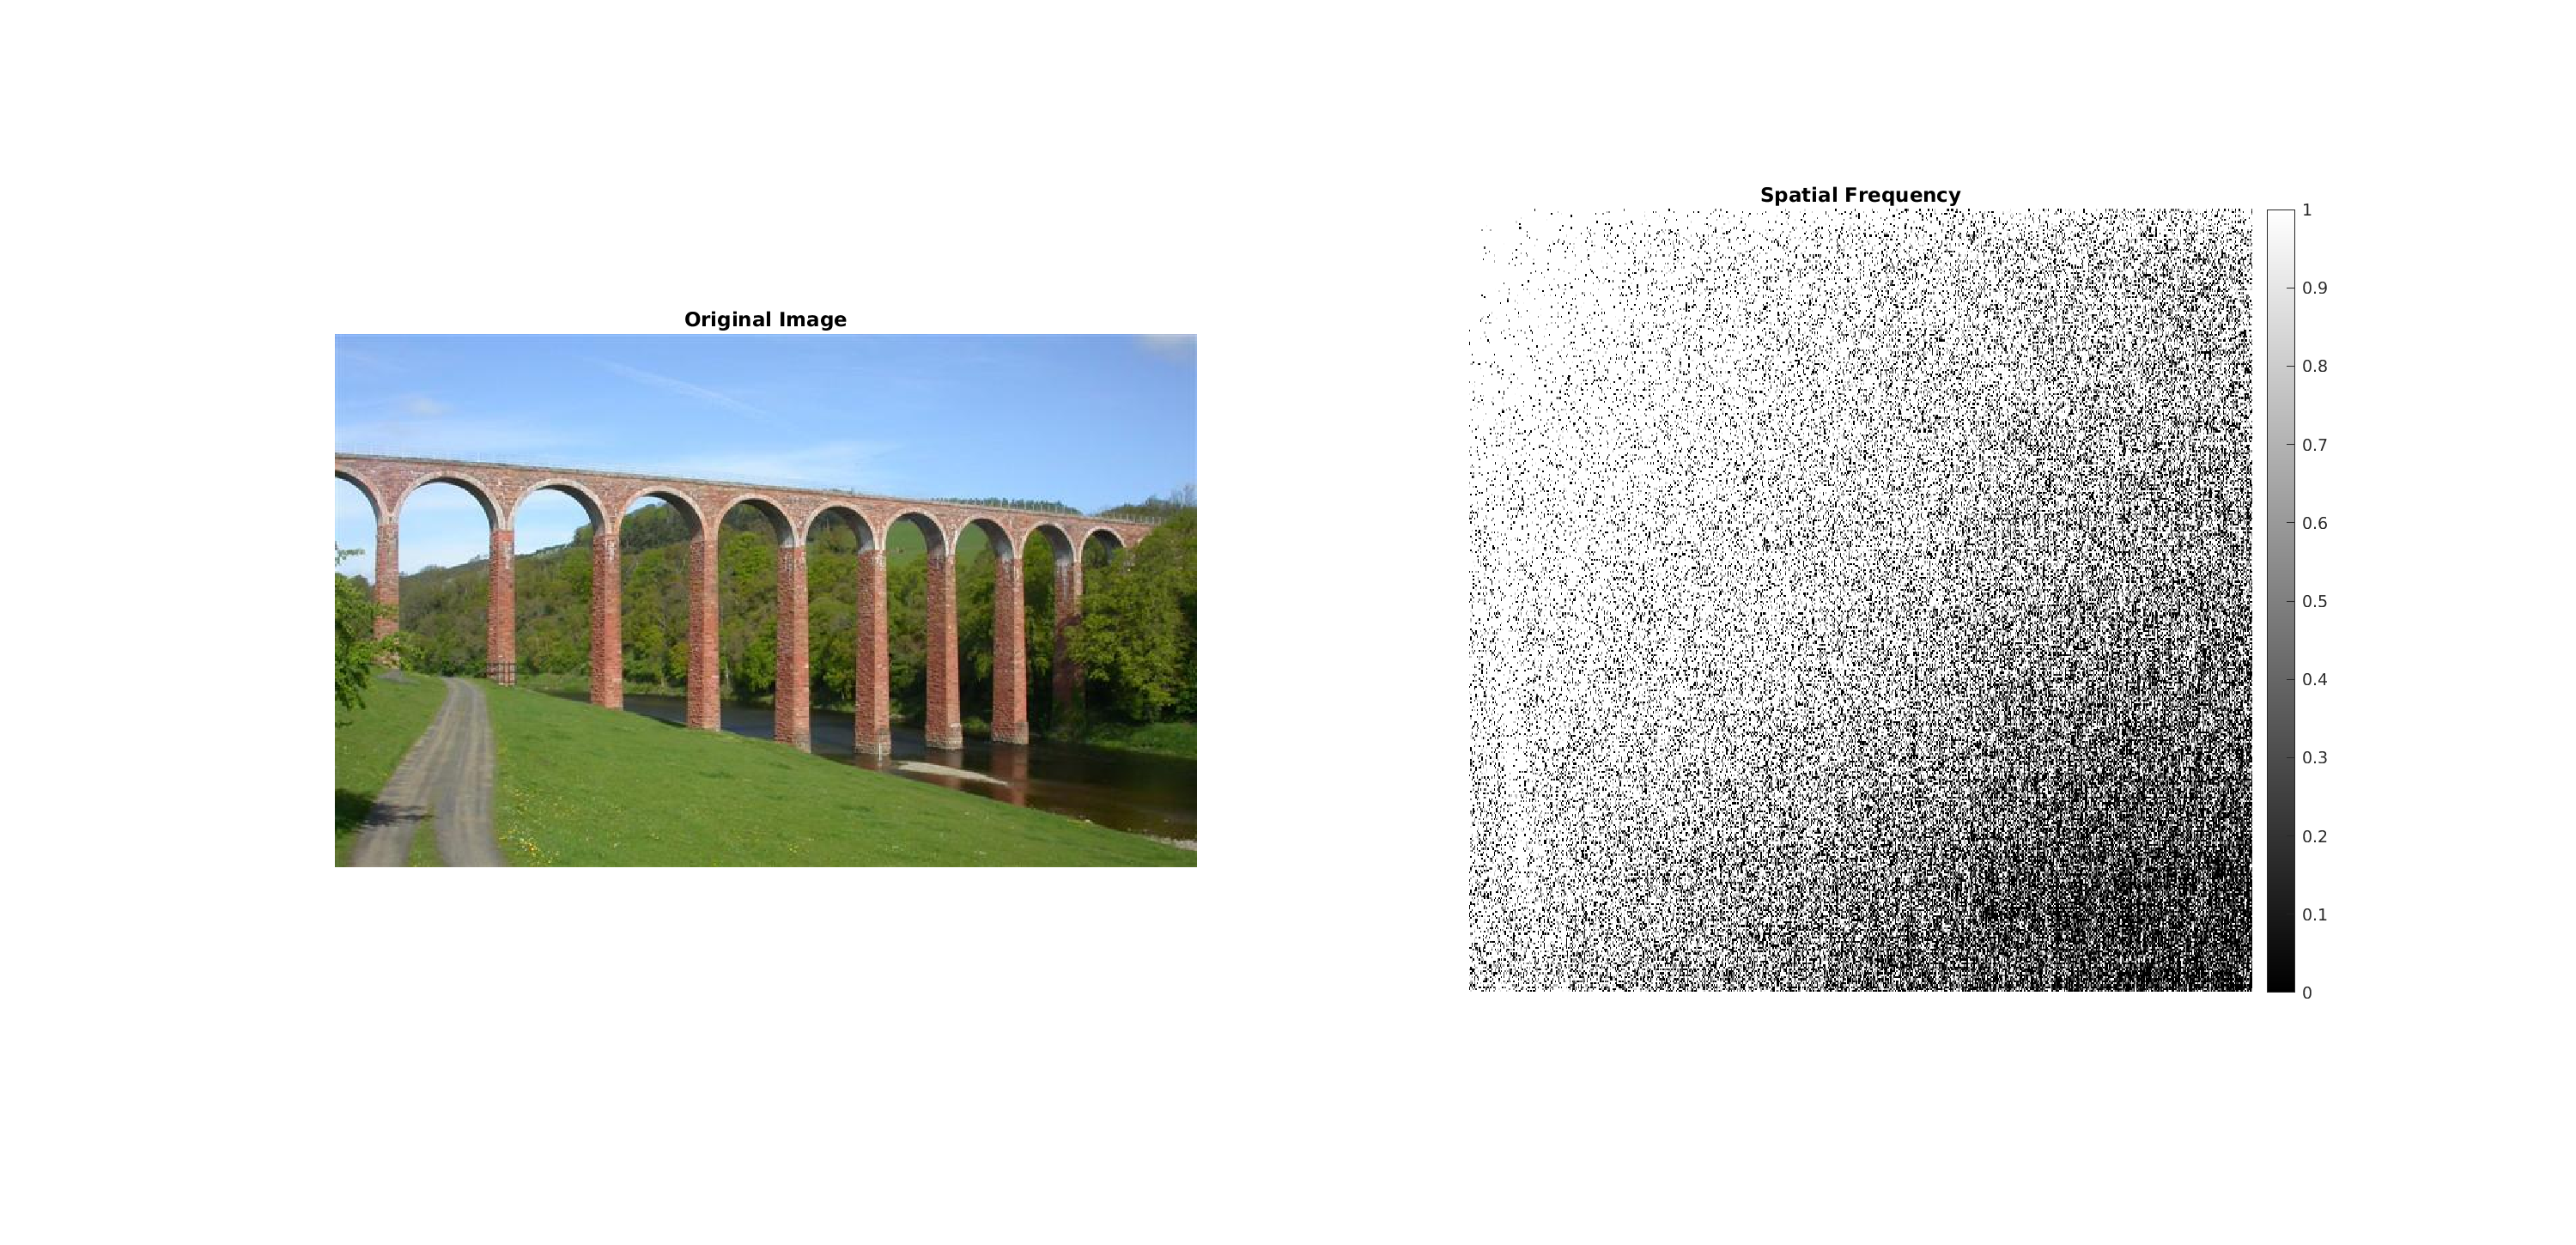
\includegraphics[width=\textwidth]
        {images/lsbrgb/dct/viaduct_medreq_dct.png}}
        \caption{\label{fig:midfreq} Mid frequency image (left) and spatial frequency distribution (right).}
      \end{figure}
      \begin{figure}[!htb]
        \center{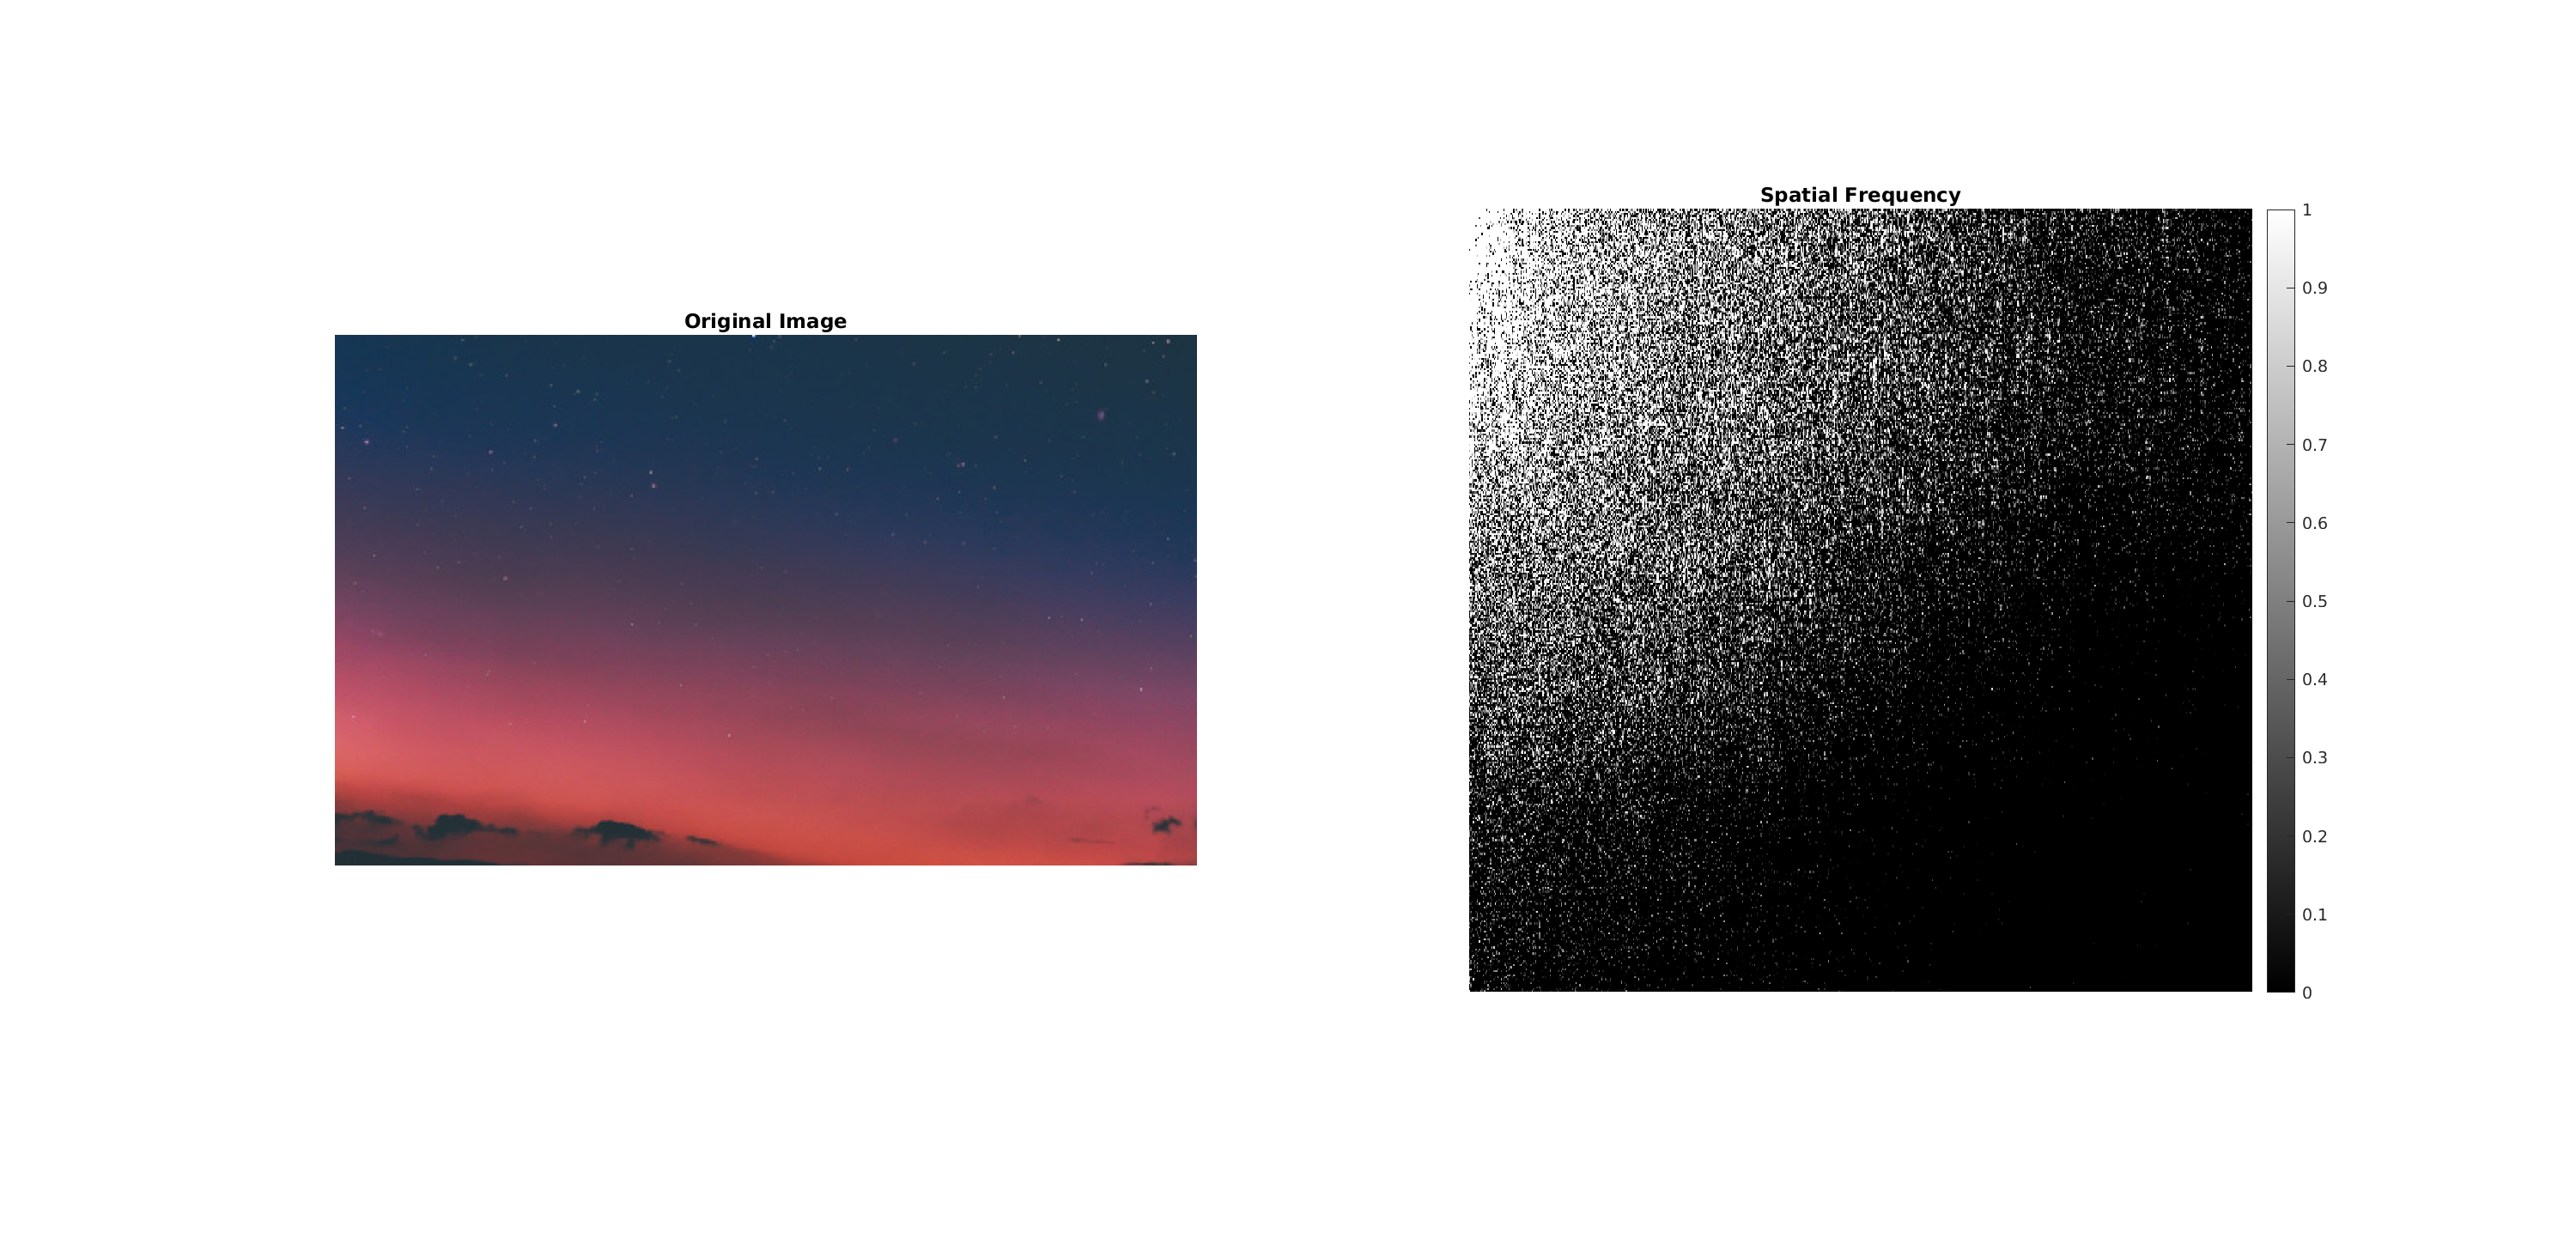
\includegraphics[width=\textwidth]
        {images/lsbrgb/dct/sky_lowfreq_dct.png}}
        \caption{\label{fig:lowfreq} Low frequency image \cite{sky} (left) and spatial frequency distribution (right)}.
      \end{figure}
      


\section{LSB with RGB and YCbCr} \label{rgbvsycbcr}

YCbCr uses values for the luminance, and red and blue chromaticities, which produces a different colour gamut to RGB. However, since the human eye is more sensitive to black and white information than to changes in colour, the number of bytes used for the Cb and Cr channels can be reduced (called chroma subsampling) without any significant effect on image perception, which means its often used for data-in-motion. Some modern approaches to steganography are based on domain transformations on YCbCr images. Bits of the message can be submitted for the coefficients of the discrete cosine transform (DCT) or Discrete Wavelet Transform (DWT) of the image \cite{maurya_shrivastava_2014} \cite{s_dinesh_acharya_a_2013}. 



\part{Penetration Testing}

\part*{Conclusion}

\bibliographystyle{unsrt}
\bibliography{mybib}

\end{document}
